% Created 2015-09-15 Tue 17:00
\documentclass{article}
\usepackage[top=1in, bottom=1.in, left=1in, right=1in]{geometry}
  \usepackage[makeroom]{cancel}
\usepackage{verbatim}


\usepackage[utf8]{inputenc}
\usepackage{lmodern}
\usepackage[T1]{fontenc}
\usepackage{fixltx2e}
\usepackage{graphicx}
\usepackage{longtable}
\usepackage{float}
\usepackage{wrapfig}
\usepackage{rotating}
\usepackage[normalem]{ulem}
\usepackage{amsmath}
\usepackage{textcomp}
\usepackage{marvosym}
\usepackage{wasysym}
\usepackage{amssymb}
\usepackage{amsmath}
\usepackage[version=3]{mhchem}
\usepackage[numbers,super,sort&compress]{natbib}
\usepackage{natmove}
\usepackage{url}
\usepackage{minted}
\usepackage{underscore}
\usepackage[linktocpage,pdfstartview=FitH,colorlinks,
linkcolor=blue,anchorcolor=blue,
citecolor=blue,filecolor=blue,menucolor=blue,urlcolor=blue]{hyperref}
\usepackage{attachfile}
\author{Abhishek Bagusetty}
\date{\today}
\title{24-623 2015 HM1}
\begin{document}

\maketitle

\section{Problem 1}
\label{sec-1}
\subsection{(i)}
\label{sec-1-1}
$$ 2x^6 - 3x^4 + 4x^2 - 3$$
For efficient calculations we can use the following,
$$  x^2 = x*x$$
$$  x^4 = x^2 * x^2$$
$$  x^6 = x^4 * x^2$$
This will minimize the number of FLOPS as well as any temporary variables created during the process.

\subsection{(ii)}
\label{sec-1-2}
Prime number is only divisible by one and itself. Hence we iterate and find any numbers that factor the variable there by tagging it as composite. Algorithm to find if a number is prime is performed by using a common \textbf{primality} algorithm :

\begin{enumerate}
\item The given number is tested if it is PERFECT SQUARE or not (the code for this is already provided). This information is used in the subsequent steps to search.
\item A set of numbers check if a given number is a factor.
\item If the number has a PERFECT SQUARE, we iterate all the numbers starting from 2 till the square of that number because the factors will be repeated anyway.
\item If the number is NOT a PERFECT SQUARE, we iterate all the number starting from 2 till the (number-1).
\item NOTE : We start iterations from 2 and only iterate odd numbers as the even numbers can already divided by 2.
\end{enumerate}

The output of the program is piped to \texttt{5output.txt}

\section{Problem 2}
\label{sec-2}
\subsection{Paper 1: (Application) Rapid transport of gases in carbon nanotubes}
\label{sec-2-1}

This paper is chosen based on the following reasons mostly focused on the applications,

\begin{enumerate}
\item The paper is interesting owing to the usage of molecular dynamics (MD) and monte-carlo (MC) techniques at various segments of the calculation.
\item MC technique has been used for sampling the phase space for equilibration and MD is used for the production calculations.
\item Usage of various concepts like equilibration, averaging techniques, usage of ensembles, etc have been made and it would be a good overview in applying to a practical system.
\item System under consideration is of enormous importance on which atomic simulations are performed to compute both the self- and transport diffusivities of light gases like $CH_4$ and $H_2$ in single walled carbon nanotubes (SWNTs) and also in zeolites with comparable pore sizes.
\item $CH_4$ and $H_2$ are treated as rigid spheres with pairwise lennard-jones interaction between species.
\item It would be of great interest to study the transport properties of the gases through the material so that better molecular sieves, membranes can be designed from the data obtained from atomistic simulations.
\item Defect-free nanotubes are considered for the calculations. The presence of defects in the nanotubes (heteroatoms, holes, etc.) will have an impact on molecular diffusion. The simplicity of the system would make it reproduce the calculations.
\item The results states that the rapid transport of adsorbed gasees in the SWNTs is not strongly dependent on the details of the adsorbate gas-nanotube interaction potentails becuase of the lack of corrugations in the PES. This would be an interesting observation to quantify.
\end{enumerate}

\subsection{Paper 2: (Theory) Application of Ewald summations to long-range dispersion forces}
\label{sec-2-2}

This paper is chosen from a theortical stand-point,

\begin{enumerate}
\item Effect of using explict summation terms for the $r^{-6}$ dispersion term on the interfacial properties of a Lennard-Jones fluid and SPC/E water is discussed in this paper.
\item At large distances r, the effect of repulsive term drops in the LJ potential term. $$u_{ij}(r) = 4\epsilon_{ij}\Big[\cancel{\Big(\frac{\sigma_{ij}}{r}\Big)^{12}} - \Big(\frac{\sigma_{ij}}{r}\Big)^6\Big]$$
\item Ewald summation technique is employed to perform summation of the pair-wise potential terms governing mostly dispersion at large-range distances and also ensuring convergence.
\item This has been widely reported in the LAMMPS and well documented which makes it interesting to study.
\end{enumerate}

\section{Problem 3}
\label{sec-3}
\subsection{(a)}
\label{sec-3-1}
Assumption : Water at NPT conditions

\uline{Some mertics}

1 mole = 6.023.1E+23 molecules, 1 lit = 1E+24 $nm^3$

\begin{center}
\begin{tabular}{rrrrr}
\hline
diameter(nm) & Volume$(nm^3)$ & moles & molecules & App. (molecules)\\
\hline
1 & 0.5238095 & 2.910052\,(-23) & 1.7527\,(+01) & 18\\
10 & 5.238095 & 2.910052\,(-22) & 1.7527\,(+02) & 180\\
100 & 52.38095 & 2.910052\,(-21) & 1.7527\,(+03) & 1800\\
\hline
\end{tabular}
\end{center}

\subsection{(b)}
\label{sec-3-2}
The number of distinct interactions when treating water as a 3-body system with rigid bonds, 
$$ n = 3[3(N-1)] \implies 9(N-1) $$ 
where n is the number of distinct pairwise interactions and N is the number of molecules involved. 

\begin{center}
\begin{tabular}{rrl}
\hline
diameter(nm) & Molecules & Interactions\\
\hline
1 & 18 & 9(18-1) = 153\\
10 & 180 & 9(180-1) = 1611\\
100 & 1800 & 9(1800-1) = 16191\\
\hline
\end{tabular}
\end{center}

\section{Problem 4}
\label{sec-4}
\subsection{(a)}
\label{sec-4-1}

\subsubsection{Equation 1 with two isolated atoms}
\label{sec-4-1-1}
\begin{equation}
u(r) = 4\epsilon \Big[\Big(\frac{\sigma}{r}\Big)^{12} - \Big(\frac{\sigma}{r}\Big)^6\Big] \label{eq:1}
\end{equation}

Change of variables from r to $r_{nn}$.
\begin{equation}
U_{i}(r_{nn}) = \frac{1}{2} \sum_{j \neq i} u(r_{ij}) \label{eq:2}
\end{equation}

Substitute \eqref{eq:1} in \eqref{eq:2}, 

\begin{equation}
U_{i}(r_{nn}) = 2\epsilon \Big[\Big(\frac{\sigma}{r_{nn}}\Big)^{12} - \Big(\frac{\sigma}{r_{nn}}\Big)^6\Big] \label{eq:3}
\end{equation}

\begin{equation}
\boxed{\frac{U_{i}(r_{nn})}{\epsilon} = 2 \Big[\Big(\frac{1}{r_{nn}/\sigma}\Big)^{12} - \Big(\frac{1}{r_{nn}/\sigma}\Big)^6\Big] \label{eq:4}}
\end{equation}

\subsubsection{Equation 3 with FCC}
\label{sec-4-1-2}
\begin{equation}
\frac{U_{i}(r_{nn})}{\epsilon} = 2 \Big[A_{12}\Big(\frac{\sigma}{r_{nn}}\Big)^{12} - A_6\Big(\frac{\sigma}{r_{nn}}\Big)^6\Big] \label{eq:5}
\end{equation}

\begin{equation}
\boxed{\frac{U_{i}(r_{nn})}{\epsilon} = 2 \Big[A_{12}\Big(\frac{1}{r_{nn}/\sigma}\Big)^{12} - A_6\Big(\frac{1}{r_{nn}/\sigma}\Big)^6\Big] \label{eq:6}}
\end{equation}

\begin{figure}[H]
\begin{centering}
\scalebox{0.75}{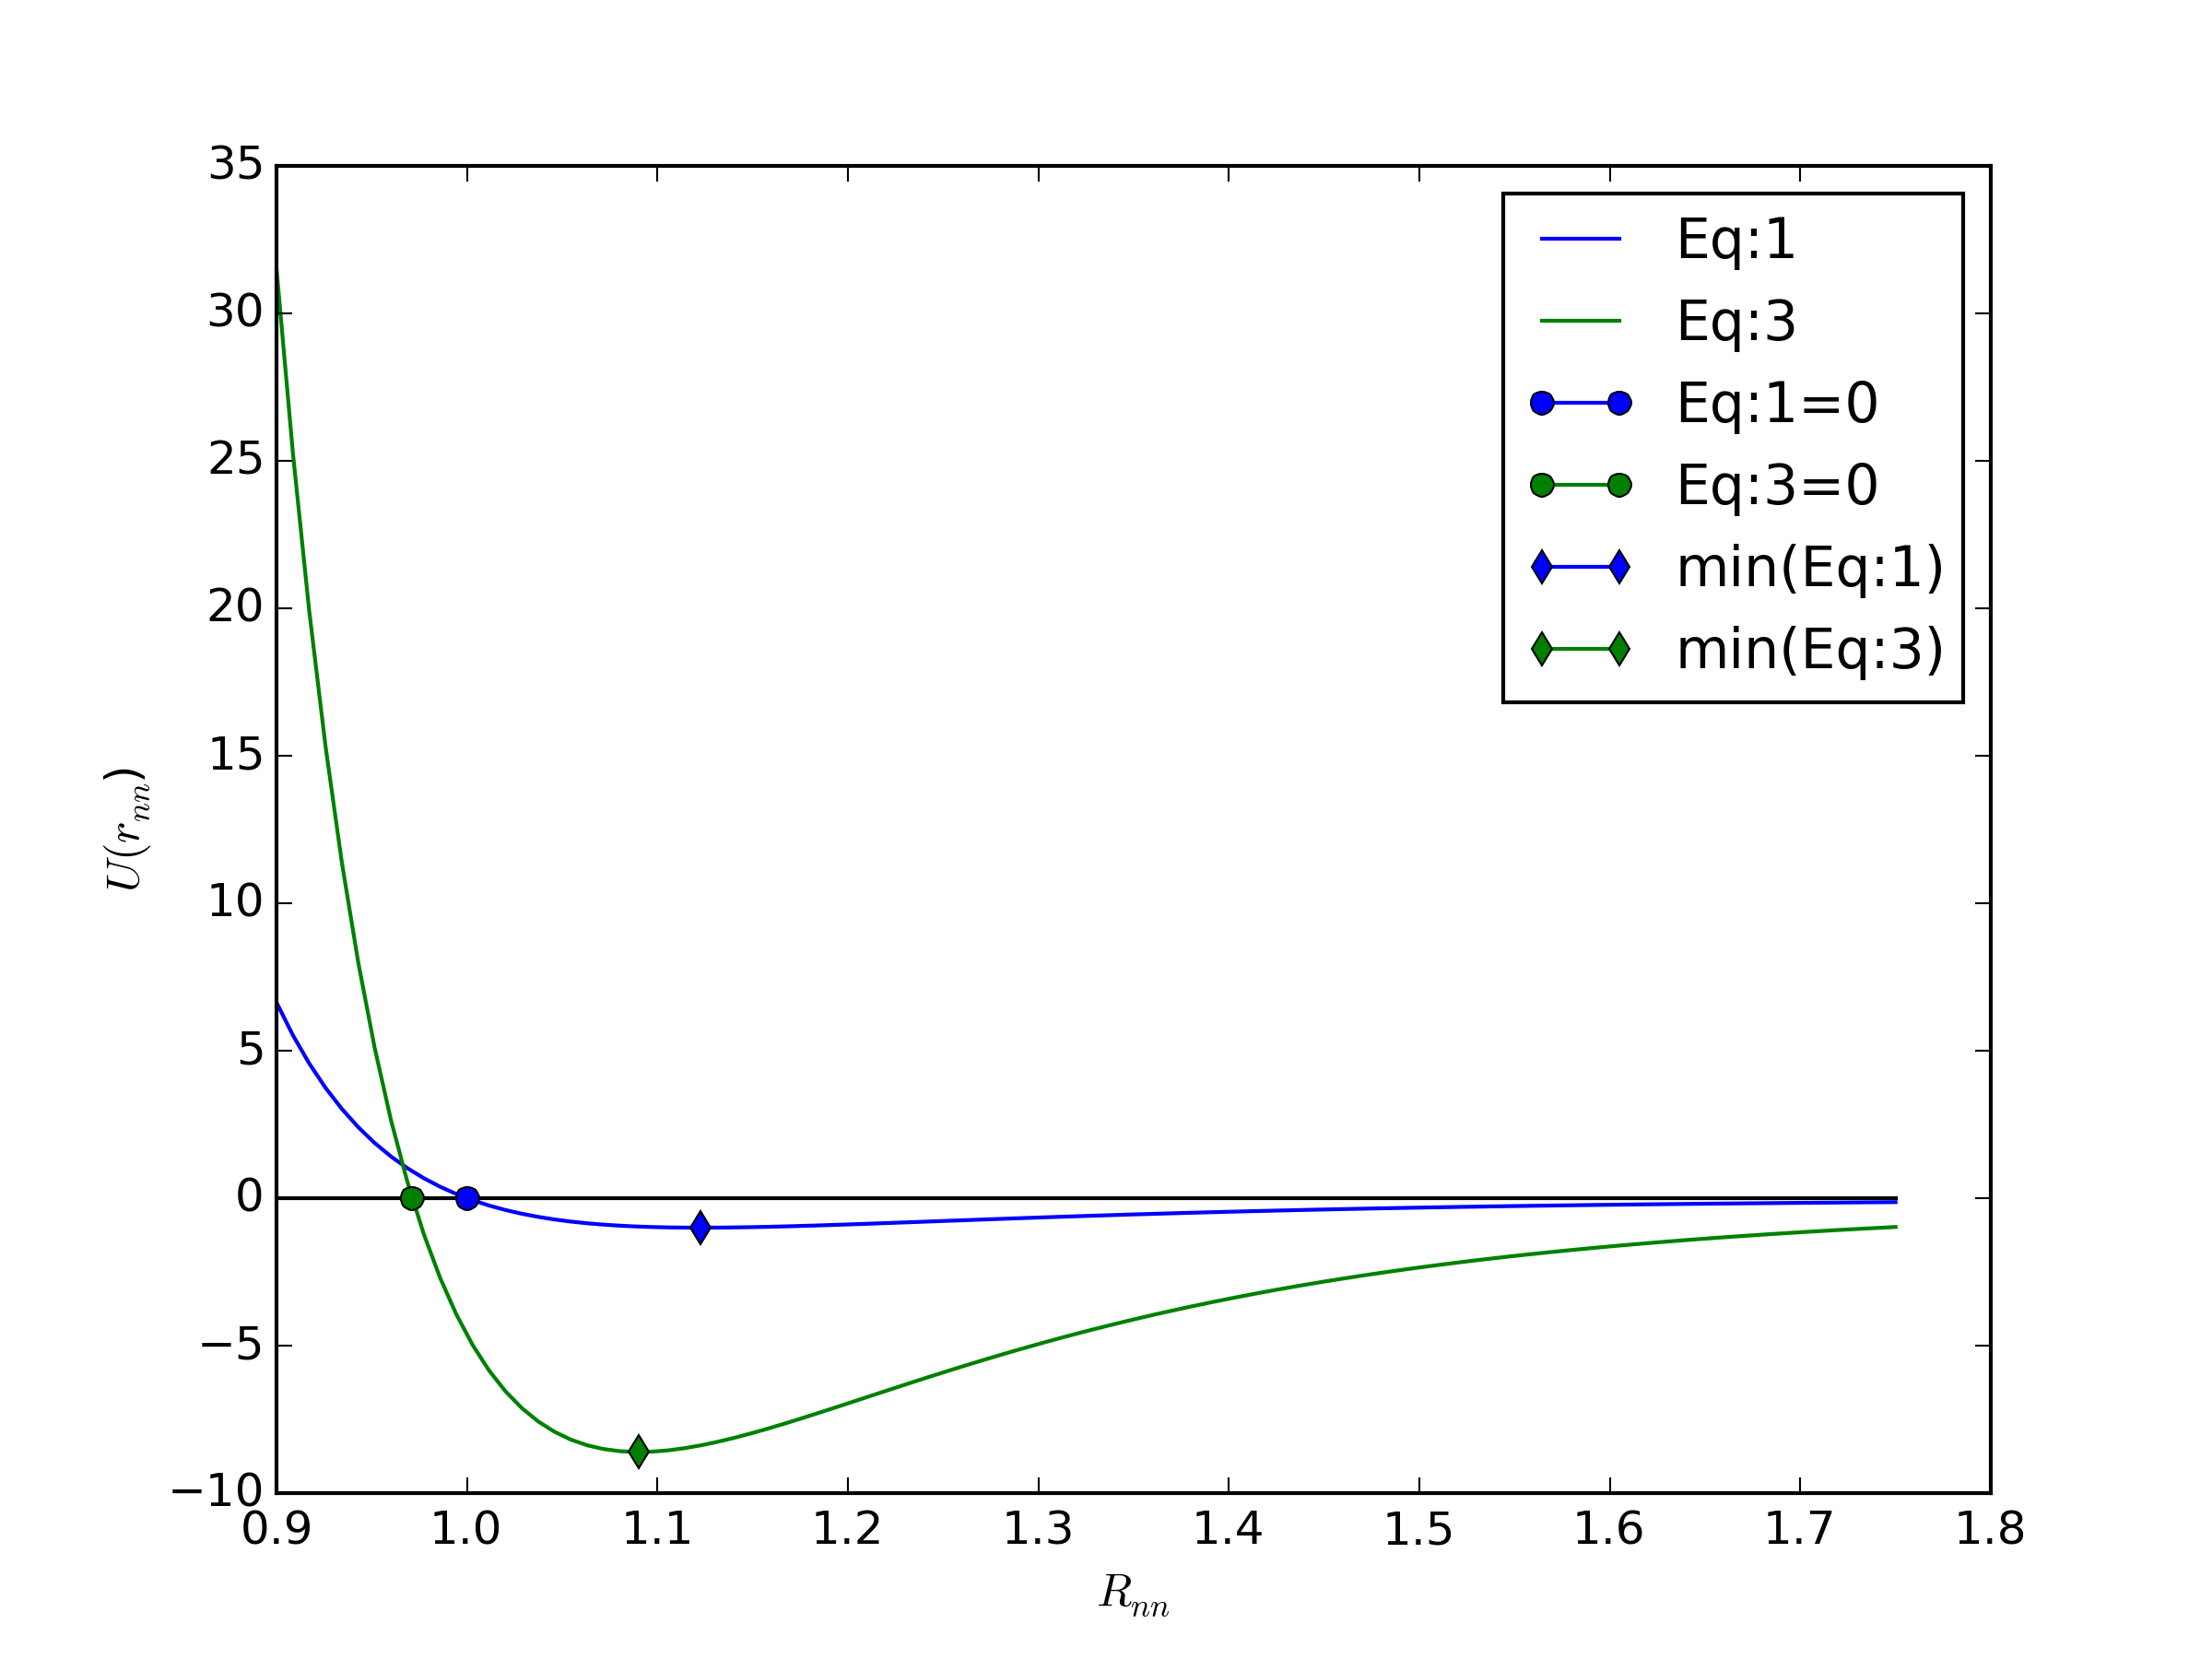
\includegraphics{./LJ-Ex4.png}}
\caption{The figure shows the plot for LJ potential without environment (blue) and with environment in FCC (green). The potential is zero at larger distance for both the cases and it is zero at the positions shown in colored circle. The minima for the potential is also shown in filled diamonds.}
\label{fig:fig1}
\end{centering}
\end{figure}

The decay of the expression is faster for the \eqref{eq:4} when compared to \eqref{eq:6}.

\subsection{(b)}
\label{sec-4-2}
\begin{equation}
\boxed{u(r) = 4\epsilon\Big[\big(\frac{\sigma}{r}\big)^{12}-\big(\frac{\sigma}{r}\big)^6\Big] \label{eq:7}}
\end{equation}

Setting u(r) = 0 in \eqref{eq:7}
$$\implies 0 = 4\epsilon\Big[\big(\frac{\sigma}{r}\big)^{12}-\big(\frac{\sigma}{r}\big)^6\Big]$$

\begin{equation}
\implies \big(\frac{\sigma}{r}\big)^6\Big[\big(\frac{\sigma}{r}\big)^6-1\Big] = 0 \label{eq:8})
\end{equation}

Roots of the \eqref{eq:8}, \underline{$r = \infty$} and \underline{$r = \sigma$}, at which $u(r)=0$.

For finding minimum for \eqref{eq:7}, set $\frac{du(r)}{dr} = 0$

\begin{equation}
\frac{du(r)}{dr} = 4\epsilon\Big[ \frac{-12\sigma^{12}}{r^{13}} + \frac{6\sigma^6}{r^7} \Big]
\end{equation}

\begin{equation}
\implies 4\epsilon\sigma^6 \Big[ \frac{-12\sigma^6}{r^{13}} + \frac{6}{r^7} \Big] = 0 \label{eq:9}
\end{equation}
$$\implies \frac{1}{r^7} \Big[ \frac{2\sigma^6}{r^6} - 1 \Big] = 0 $$

Root of \eqref{eq:9}, $r=\infty$ and $r = \qquad \sigma\sqrt[\leftroot{-1}\uproot{2}\scriptstyle 6]2\qquad$ at which $u(r)$ is at minimum.

\begin{equation}
\boxed{U_i(r_{nn}) = 2\epsilon\Big[A_{12}\Big(\frac{\sigma}{r_{nn}}\Big)^{12} - A_6\Big(\frac{\sigma}{r_{nn}}\Big)^6\Big] \label{eq:10}}
\end{equation}

Setting $U_i(r_{nn})$ = 0 in \eqref{eq:11}
$$\implies 0 =
2\epsilon\Big[A_{12}\Big(\frac{\sigma}{r_{nn}}\Big)^{12}-A_6\Big(\frac{\sigma}{r_{nn}}\Big)^6\Big] $$

\begin{equation}
\implies 2\epsilon\Big(\frac{\sigma^6}{r_{nn}}\Big) \Big[A_{12}\Big(\frac{\sigma}{r_{nn}}\Big)^{6} - A_6\Big] = 0 \label{eq:11}
\end{equation}

Roots of the \eqref{eq:12}, $r_{nn} = \infty$ and
$r_{nn} = \qquad \sigma \sqrt[\leftroot{-1}\uproot{2}\scriptstyle 6]{\frac{A_{12}}{A_6}}\qquad$ at which $U(r_{nn})=0$.

\newline
For finding minimum for \eqref{eq:11}, set $\frac{dU_i(r_{nn})}{dr_{nn}} = 0$

\begin{equation}
\frac{dU_i(r_{nn})}{dr_{nn}} = 2\epsilon\Big[ A_{12}\frac{-12\sigma^{12}}{r_{nn}^{13}} + A_6\frac{6\sigma^6}{r_{nn}^7} \Big]
\end{equation}

$$\implies -12\frac{\epsilon\sigma^6}{r_{nn}^7} \Big[ A_{12}\frac{\sigma^6}{r_{nn}^6} - A_6 \Big] = 0$$

\begin{equation}
\implies \frac{1}{r_{nn}^7} \Big[ A_{12}\frac{\sigma^6}{r_{nn}^6} - A_6 \Big] = 0 \label{eq:12}
\end{equation}

Root of \eqref{eq:12}, $r_{nn}=\infty$ and $r_{nn} = \qquad \sigma\sqrt[\leftroot{-1}\uproot{2}\scriptstyle 6]{\frac{2A_{12}}{A_6}}\qquad$ at which $U_i(r_{nn})$ is at minimum.

The plot of these singularity and minima is shown in the Figure.\ref{fig:fig1}

\subsection{(c)}
\label{sec-4-3}
$k_{LJ}$ is dimnesionless LJ thermal conductivity,

$$\boxed{k_{LJ} = \frac{k_B}{\sigma^2} \sqrt{\frac{\epsilon}{m}}}$$

\subsection{(d)}
\label{sec-4-4}
dimensionless temperature $(T^{*})$, 
$$ T = T^{*} \Big(\frac{\epsilon}{k_B}\Big) \implies T^{*} = \frac{T}{\epsilon/k_B} $$

dimensionless thermal conductivity $(k^{*})$, 
$$k = k^{*}\Big(\frac{k_B}{\sigma^2}\sqrt{\frac{\epsilon}{m}}\Big) \implies k^* = \frac{k}{\Big(\frac{k_B}{\sigma^2}\sqrt{\frac{\epsilon}{m}}\Big)}$$

\uline{Argon}
\subsubsection{Dimensionless Temperature}
\label{sec-4-4-1}
$$T^* = \frac{20K}{\frac{1.67.1E{-21}J}{1.3806.1E^{-23}J/K}}$$
$$\boxed{T^*_{Argon} = 0.1653}$$
\subsubsection{Dimensionless thermal conductivity}
\label{sec-4-4-2}
$$k^* = \frac{1.4W/m-K}{\Big(\frac{1.3806.1E-23J/K}{(3.4.1E-10 m)^2}\sqrt{\frac{1.67.1E-21J}{6.63.1E-26 kg}}\Big)} $$
$$\boxed{k_{Argon}^{*} = 0.018955} $$
\uline{Krypton}
\subsubsection{Corresponding Temperature}
\label{sec-4-4-3}
$$T_{krypton} = T^*_{Argon} \Big(\epsilon/k_B\Big)$$
$$T = 0.1653K \Big(\frac{1.67.1E{-21}J}{1.3806.1E{-23}J/K}\Big)$$
$$\boxed{T_{krypton} = 26.82K}$$
\subsubsection{Corresponding Thermal conductivity}
\label{sec-4-4-4}
$$k_{krypton} = k^*_{argon}\Big(\frac{k_B}{\sigma^2}\sqrt{\frac{\epsilon}{m}}\Big)$$

$$k = 0.018955 \Big(\frac{1.3806.1E-23J/K}{(3.65.1E-10 m)^2}\sqrt{\frac{2.24.1E-21J}{13.9.1E-26 kg}}\Big) $$

$$\boxed{k_{krypton} = 2.4935.1E-4   W/m-K} $$

\bibliographystyle{unsrt}

\bibliography{/Users/abhimac/Box Sync/Classes/CMUME24623-MolSim_Materials-Fall2015/HM1/references}
% Emacs 24.4.1 (Org mode 8.2.10)
\end{document}